\documentclass[conference]{IEEEtran}
\usepackage{amsmath,amssymb,booktabs,graphicx,xcolor,cite,url,siunitx,microtype,adjustbox}
\usepackage[hidelinks]{hyperref}
% generated by scripts/make_paper_assets.py -- do not edit
\newcommand{\nRaw}{8{,}000}
\newcommand{\nClean}{7{,}969}
\newcommand{\nDropped}{31}
\newcommand{\nFlagged}{550}
\newcommand{\flaggedPct}{6.9\,\%}
\newcommand{\nGroups}{7{,}812}
\newcommand{\randLeakGroups}{41}
\newcommand{\randLeakPct}{2.7\,\%}
\newcommand{\resOnlyAcc}{96.8\,\%}
\newcommand{\resGeomAcc}{99.3\,\%}
\newcommand{\regionMajority}{62.4\,\%}
\newcommand{\resGeomF}{0.34}
\newcommand{\tealCecum}{95\,\%}
\newcommand{\vifMedian}{220}
\newcommand{\nVifTen}{79}
\newcommand{\acDice}{0.406}
\newcommand{\ellDice}{0.375}
\newcommand{\defDice}{0.366}
\newcommand{\fovDice}{0.272}
\newcommand{\acDiceLo}{0.373}
\newcommand{\acDiceHi}{0.440}
\newcommand{\acIoU}{0.281}
\newcommand{\acDelta}{+0.031}
\newcommand{\acDeltaLo}{+0.019}
\newcommand{\acDeltaHi}{+0.042}
\newcommand{\acWilcoxP}{$2.5{\times}10^{-6}$}
\newcommand{\acBetterFrac}{62\,\%}
\newcommand{\acNtest}{176}
\newcommand{\acOverSeg}{2.4}
\newcommand{\acDiceSmall}{0.21}
\newcommand{\acDiceMed}{0.45}
\newcommand{\acDiceLarge}{0.62}
\newcommand{\resnetF}{0.8708}
\newcommand{\resnetFSD}{0.0043}
\newcommand{\resnetAcc}{0.8712}
\newcommand{\resnetAccSD}{0.0045}
\newcommand{\resnetAU}{0.9916}
\newcommand{\resnetAUSD}{0.0017}
\newcommand{\resnetECE}{0.0300}
\newcommand{\resnetECESD}{0.0026}
\newcommand{\effnetF}{0.9257}
\newcommand{\effnetFSD}{0.0025}
\newcommand{\effnetAcc}{0.9258}
\newcommand{\effnetAccSD}{0.0025}
\newcommand{\effnetAU}{0.9957}
\newcommand{\effnetAUSD}{0.0004}
\newcommand{\effnetECE}{0.0256}
\newcommand{\effnetECESD}{0.0035}
\newcommand{\convnextF}{0.9233}
\newcommand{\convnextFSD}{0.0006}
\newcommand{\convnextAcc}{0.9235}
\newcommand{\convnextAccSD}{0.0006}
\newcommand{\convnextAU}{0.9931}
\newcommand{\convnextAUSD}{0.0029}
\newcommand{\convnextECE}{0.0353}
\newcommand{\convnextECESD}{0.0027}
\newcommand{\swinF}{0.9327}
\newcommand{\swinFSD}{0.0045}
\newcommand{\swinAcc}{0.9327}
\newcommand{\swinAccSD}{0.0045}
\newcommand{\swinAU}{0.9947}
\newcommand{\swinAUSD}{0.0014}
\newcommand{\swinECE}{0.0306}
\newcommand{\swinECESD}{0.0050}
\newcommand{\dinoF}{0.9344}
\newcommand{\dinoFSD}{0.0058}
\newcommand{\dinoAcc}{0.9343}
\newcommand{\dinoAccSD}{0.0058}
\newcommand{\dinoAU}{0.9916}
\newcommand{\dinoAUSD}{0.0015}
\newcommand{\dinoECE}{0.0242}
\newcommand{\dinoECESD}{0.0035}
\newcommand{\resacgF}{0.8560}
\newcommand{\resacgFSD}{0.0103}
\newcommand{\resacgAcc}{0.8565}
\newcommand{\resacgAccSD}{0.0100}
\newcommand{\resacgAU}{0.9887}
\newcommand{\resacgAUSD}{0.0023}
\newcommand{\resacgECE}{0.0353}
\newcommand{\resacgECESD}{0.0049}
\newcommand{\lgbGF}{0.751}
\newcommand{\lgbGAcc}{0.751}
\newcommand{\lgbGAU}{0.957}
\newcommand{\lgbACF}{0.806}
\newcommand{\lgbACAcc}{0.807}
\newcommand{\lgbACAU}{0.972}
\newcommand{\lgbGACF}{0.795}
\newcommand{\lgbGACAcc}{0.796}
\newcommand{\lgbGACAU}{0.972}
\newcommand{\lrGACF}{0.776}
\newcommand{\lrGACAcc}{0.777}
\newcommand{\lrGACAU}{0.971}
\newcommand{\lgbGEllF}{0.800}
\newcommand{\lgbGEllAcc}{0.801}
\newcommand{\lgbGEllAU}{0.979}
\newcommand{\lgbGShufF}{0.784}
\newcommand{\lgbGShufAcc}{0.785}
\newcommand{\lgbGShufAU}{0.970}
\newcommand{\svmGACF}{0.790}
\newcommand{\svmGACAcc}{0.790}
\newcommand{\svmGACAU}{0.975}
\newcommand{\rfGACF}{0.766}
\newcommand{\rfGACAcc}{0.767}
\newcommand{\rfGACAU}{0.962}
\newcommand{\xgbGACF}{0.795}
\newcommand{\xgbGACAcc}{0.795}
\newcommand{\xgbGACAU}{0.973}
\newcommand{\dinoProbeF}{0.889}
\newcommand{\dinoProbeAcc}{0.889}
\newcommand{\dinoProbeAU}{0.995}
\newcommand{\randF}{0.131}
\newcommand{\randAU}{0.495}
\newcommand{\priorF}{0.028}
\newcommand{\priorAU}{0.492}
\newcommand{\heurF}{0.476}
\newcommand{\heurAU}{0.837}
\newcommand{\plainF}{0.9233}
\newcommand{\plainFSD}{0.0006}
\newcommand{\plainAcc}{0.9235}
\newcommand{\plainAccSD}{0.0006}
\newcommand{\plainAU}{0.9931}
\newcommand{\plainAUSD}{0.0029}
\newcommand{\gfeatF}{0.9295}
\newcommand{\gfeatFSD}{0.0035}
\newcommand{\gfeatAcc}{0.9295}
\newcommand{\gfeatAccSD}{0.0035}
\newcommand{\gfeatAU}{0.9927}
\newcommand{\gfeatAUSD}{0.0020}
\newcommand{\gfeatDelta}{+0.0062}
\newcommand{\gfeatDeltaLo}{+0.0013}
\newcommand{\gfeatDeltaHi}{+0.0111}
\newcommand{\gfeatPHolm}{0.072}
\newcommand{\gfeatPMcnemar}{0.031}
\newcommand{\acpoolF}{0.9264}
\newcommand{\acpoolFSD}{0.0037}
\newcommand{\acpoolAcc}{0.9264}
\newcommand{\acpoolAccSD}{0.0038}
\newcommand{\acpoolAU}{0.9934}
\newcommand{\acpoolAUSD}{0.0010}
\newcommand{\acpoolDelta}{+0.0031}
\newcommand{\acpoolDeltaLo}{$-$0.0015}
\newcommand{\acpoolDeltaHi}{+0.0075}
\newcommand{\acpoolPHolm}{0.380}
\newcommand{\acpoolPMcnemar}{0.143}
\newcommand{\acfeatF}{0.9288}
\newcommand{\acfeatFSD}{0.0003}
\newcommand{\acfeatAcc}{0.9289}
\newcommand{\acfeatAccSD}{0.0004}
\newcommand{\acfeatAU}{0.9932}
\newcommand{\acfeatAUSD}{0.0015}
\newcommand{\acfeatDelta}{+0.0055}
\newcommand{\acfeatDeltaLo}{+0.0004}
\newcommand{\acfeatDeltaHi}{+0.0106}
\newcommand{\acfeatPHolm}{0.180}
\newcommand{\acfeatPMcnemar}{0.076}
\newcommand{\acgF}{0.9277}
\newcommand{\acgFSD}{0.0035}
\newcommand{\acgAcc}{0.9279}
\newcommand{\acgAccSD}{0.0035}
\newcommand{\acgAU}{0.9900}
\newcommand{\acgAUSD}{0.0013}
\newcommand{\acgDelta}{+0.0045}
\newcommand{\acgDeltaLo}{$-$0.0004}
\newcommand{\acgDeltaHi}{+0.0091}
\newcommand{\acgPHolm}{0.296}
\newcommand{\acgPMcnemar}{1.000}
\newcommand{\shufF}{0.9275}
\newcommand{\shufFSD}{0.0015}
\newcommand{\shufAcc}{0.9276}
\newcommand{\shufAccSD}{0.0016}
\newcommand{\shufAU}{0.9912}
\newcommand{\shufAUSD}{0.0028}
\newcommand{\shufDelta}{+0.0043}
\newcommand{\shufDeltaLo}{$-$0.0010}
\newcommand{\shufDeltaHi}{+0.0093}
\newcommand{\shufPHolm}{0.354}
\newcommand{\shufPMcnemar}{0.248}
\newcommand{\ellF}{0.9267}
\newcommand{\ellFSD}{0.0067}
\newcommand{\ellAcc}{0.9268}
\newcommand{\ellAccSD}{0.0067}
\newcommand{\ellAU}{0.9908}
\newcommand{\ellAUSD}{0.0026}
\newcommand{\ellDelta}{+0.0035}
\newcommand{\ellDeltaLo}{$-$0.0017}
\newcommand{\ellDeltaHi}{+0.0085}
\newcommand{\ellPHolm}{0.380}
\newcommand{\ellPMcnemar}{0.585}
\newcommand{\naiveF}{0.9248}
\newcommand{\naiveFSD}{0.0048}
\newcommand{\naiveAU}{0.9936}
\newcommand{\randsplitF}{0.9356}
\newcommand{\randsplitFSD}{0.0037}
\newcommand{\randsplitAU}{0.9994}
\newcommand{\robPlainClean}{0.917}
\newcommand{\robPlainJpegFifty}{0.901}
\newcommand{\robPlainJpegTen}{0.786}
\newcommand{\robPlainBlurThree}{0.848}
\newcommand{\robGfeatClean}{0.927}
\newcommand{\robGfeatJpegFifty}{0.922}
\newcommand{\robGfeatJpegTen}{0.818}
\newcommand{\robGfeatBlurThree}{0.856}
\newcommand{\robAcgClean}{0.924}
\newcommand{\robAcgJpegFifty}{0.930}
\newcommand{\robAcgJpegTen}{0.831}
\newcommand{\robAcgBlurThree}{0.879}
\newcommand{\robShufClean}{0.924}
\newcommand{\robShufJpegFifty}{0.926}
\newcommand{\robShufJpegTen}{0.835}
\newcommand{\robShufBlurThree}{0.845}
\newcommand{\robEllClean}{0.922}
\newcommand{\robEllJpegFifty}{0.930}
\newcommand{\robEllJpegTen}{0.841}
\newcommand{\robEllBlurThree}{0.873}
\newcommand{\robN}{480}
\newcommand{\lrNoneHalf}{0.9168}
\newcommand{\lrNoneDef}{0.9227}
\newcommand{\lrNoneDouble}{0.9265}
\newcommand{\lrAcgHalf}{0.9240}
\newcommand{\lrAcgDef}{0.9315}
\newcommand{\lrAcgDouble}{0.9385}
\newcommand{\lcNoneTen}{0.8473}
\newcommand{\lcNoneTwentyFive}{0.8923}
\newcommand{\lcNoneFifty}{0.9185}
\newcommand{\lcNoneFull}{0.9233}
\newcommand{\lcAcgTen}{0.8439}
\newcommand{\lcAcgTwentyFive}{0.8997}
\newcommand{\lcAcgFifty}{0.9198}
\newcommand{\lcAcgFull}{0.9277}
\newcommand{\eceRaw}{0.046}
\newcommand{\eceCal}{0.033}
\newcommand{\confCovVal}{92.9\,\%}
\newcommand{\confCov}{95.2\,\%}
\newcommand{\confCovSD}{1.1\,\%}
\newcommand{\confSize}{1.06}
\newcommand{\confSingle}{94\,\%}
\newcommand{\costHalf}{0.040}
\newcommand{\costYouden}{0.037}
\newcommand{\costOpt}{0.034}
\newcommand{\sensHalf}{94.1\,\%}
\newcommand{\specHalf}{99.6\,\%}
\newcommand{\sensYouden}{94.8\,\%}
\newcommand{\specYouden}{99.4\,\%}
\newcommand{\accColonScope}{95.0\,\%}
\newcommand{\accUpperScope}{88.4\,\%}
\newcommand{\accBox}{96.0\,\%}
\newcommand{\accNoBox}{90.8\,\%}
\newcommand{\worstClassAcc}{80.4\,\%}
\newcommand{\nErrors}{117}
\newcommand{\errRate}{7.3\,\%}
\newcommand{\errFlagged}{53\,\%}
\newcommand{\corrFlagged}{5\,\%}
\newcommand{\errPairs}{73\,\%}
\newcommand{\ensF}{0.9385}
\newcommand{\ensAcc}{0.9385}
\newcommand{\plainPoint}{84\,\%}
\newcommand{\plainCamIoU}{0.348}
\newcommand{\plainCamInAC}{65\,\%}
\newcommand{\acgPoint}{80\,\%}
\newcommand{\acgCamIoU}{0.327}
\newcommand{\acgCamInAC}{68\,\%}
\newcommand{\lrTwoPlain}{0.9311}
\newcommand{\lrTwoPlainSD}{0.0040}
\newcommand{\lrTwoAcg}{0.9322}
\newcommand{\lrTwoAcgSD}{0.0055}
\newcommand{\lrTwoDelta}{+0.0011}
\newcommand{\lrTwoLo}{$-$0.0032}
\newcommand{\lrTwoHi}{+0.0055}
\newcommand{\lrTwoP}{0.63}
\newcommand{\shapGlobal}{32\,\%}
\newcommand{\shapShape}{6\,\%}
\newcommand{\shapBoundary}{3\,\%}
\newcommand{\shapRegion}{58\,\%}
\newcommand{\lwPreFour}{0.890}
\newcommand{\lwFtFour}{0.921}
\newcommand{\lwPreThree}{0.871}
\newcommand{\lwFtThree}{0.915}
\newcommand{\lwPreOne}{0.819}
\newcommand{\lwFtOne}{0.814}

\graphicspath{{figures/}}
\sisetup{detect-all}

\begin{document}
\title{Active-Contour-Guided Feature Extraction for Endoscopic Finding and Polyp Classification:\\ A Leakage-Audited, Shortcut-Aware Study on Kvasir}
\author{%
\IEEEauthorblockN{P. Vishnu Vardhan Reddy}
\IEEEauthorblockA{Dept.\ of Computer Science and Engineering\\
Amrita Vishwa Vidyapeetham, Bangalore Campus\\
Bangalore, India\\
BL.SC.U4CSE24034@blr.students.amrita.edu}
\and
\IEEEauthorblockN{V. Guru Puneeth Reddy}
\IEEEauthorblockA{Dept.\ of Computer Science and Engineering\\
Amrita Vishwa Vidyapeetham, Bangalore Campus\\
Bangalore, India\\
BL.SC.U4CSE24056@blr.students.amrita.edu}
\and
\IEEEauthorblockN{D. Greeshmanth Reddy}
\IEEEauthorblockA{Dept.\ of Computer Science and Engineering\\
Amrita Vishwa Vidyapeetham, Bangalore Campus\\
Bangalore, India\\
BL.SC.U4CSE24067@blr.students.amrita.edu}}
\maketitle

\begin{abstract}
Classification of endoscopic findings is routinely benchmarked on Kvasir, a single-centre dataset without patient identifiers whose frames carry acquisition artefacts.
We audit Kvasir~v2 (\nDropped{} duplicate frames including one file filed under two classes; \flaggedPct{} suspected label errors; native resolution alone predicts upper-GI versus colon with \resOnlyAcc{} accuracy),
build a leakage-aware scene-grouped split, and ask whether an \emph{unsupervised} active-contour prior still helps a strong fine-tuned network.
A two-stage morphological Chan--Vese / geodesic contour, tuned on training-matched Kvasir-SEG masks, reaches a Dice of \acDice{} against \ellDice{} for a central ellipse.
Fed into ACGNet, a head that pools backbone features inside and outside the contour and fuses 98 contour features, it yields macro-F1 \acgF{} against \plainF{} for plain ConvNeXt-T
($\Delta=$ \acgDelta{}, 95\,\% CI \acgDeltaLo{} to \acgDeltaHi{}, Holm $p=$ \acgPHolm{}): \textbf{not a statistically supported gain}, and controls using shuffled-image contours or a central ellipse perform the same.
Five fine-tuned backbones reach macro-F1 \resnetF{}--\dinoF{} and a soft-voting ensemble \ensF{}; polyp-vs-rest AUROC exceeds 0.99.
Metadata shortcuts gave no measurable accuracy advantage, whereas a naive random split inflated polyp AUROC to \randsplitAU{}.
\errPairs{} of errors fall in two confusable class pairs and \errFlagged{} involve flagged labels, so label ambiguity bounds attainable accuracy.
Temperature scaling lowers ECE from \eceRaw{} to \eceCal{}, and group-aware split-conformal sets reach \confCov{} coverage at a 95\,\% target.
Code, audited splits, 48 tests and a local demo are released; Kvasir remains restricted to research and education.
\end{abstract}

\begin{IEEEkeywords}
polyp classification, active contours, Chan--Vese, endoscopy, Kvasir, shortcut learning, calibration, conformal prediction
\end{IEEEkeywords}

\section{Introduction}
Colorectal cancer prevention relies on finding and removing polyps during colonoscopy, yet adenoma detection varies
between endoscopists~\cite{pogorelov2017kvasir}. Computer-aided classification of endoscopic findings is therefore an
active research topic, and the Kvasir dataset~\cite{pogorelov2017kvasir} has become a common benchmark: 8{,}000
frames from one Norwegian hospital, evenly split over three anatomical landmarks, three pathological findings and two
polyp-removal classes.

Two observations motivate this work. First, \emph{benchmark numbers on Kvasir are rarely comparable}: public
results use different class subsets, random frame-level splits and different preprocessing, and the dataset ships
no patient or video identifiers. We show that its frames carry strong acquisition shortcuts. Native image
resolution alone, without a single pixel, separates upper-GI from colon frames with \resOnlyAcc{} accuracy, and a
picture-in-picture endoscope-position box occurs in \tealCecum{} of cecum frames and in no upper-GI frame.
Second, \emph{active contours}~\cite{kass1988snakes,chan2001active} are a classical, label-free way of delineating
a lesion candidate, and are still studied for colonoscopy segmentation~\cite{ismail2022ways}, but it is unclear
whether such a weak, unsupervised spatial prior still helps a modern pretrained network.

We therefore ask a deliberately sceptical question: \emph{does an unsupervised active-contour prior improve
a strong fine-tuned backbone, and if so, through which mechanism?} Our contributions are:
\begin{enumerate}
\item \textbf{A verified data audit} of Kvasir~v2: a label-contradicting duplicate and 30 further duplicate pairs, 6.9\,\% suspected label noise,
 shortcut quantification, and a scene-grouped leakage-aware split (Section~\ref{sec:data}).
\item \textbf{A label-free contour pipeline}: artefact-masked field-of-view canonicalisation, a two-stage
 morphological Chan--Vese / geodesic active contour tuned against expert masks on training-matched frames only,
 and 136 interpretable shape, boundary and region features (Section~\ref{sec:ac}).
\item \textbf{ACGNet}, a backbone head that pools features inside and outside the contour and fuses contour
 features, together with \emph{controls} (shuffled-image contours, a central ellipse, extra non-contour features)
 that separate ``a mask'' from ``this image's contour'' (Section~\ref{sec:acg}).
\item \textbf{A rigorous evaluation protocol}: multi-seed runs, paired bootstrap, McNemar and DeLong tests with
 Holm correction, calibration, split-conformal prediction, error and subgroup analysis, and learning curves.
\item \textbf{An open, tested, one-command reproducible package} with a local web demo.
\end{enumerate}

\section{Related Work}
\paragraph{Gastrointestinal datasets.}
Kvasir~\cite{pogorelov2017kvasir} introduced 8 expert-labelled classes; Kvasir-SEG~\cite{jha2020kvasirseg} added 1{,}000
polyp frames with expert masks, and HyperKvasir~\cite{borgli2020hyperkvasir} scaled the collection to 110{,}079 images
and 374 videos from the same hospital. For video-derived collections, grouping frames by video is already
recommended to avoid inflated test scores from near-identical neighbouring frames; Kvasir~v2 provides no such
identifiers, which is why we construct scene groups from embedding similarity (Section~\ref{sec:data}).
Reported accuracies on Kvasir vary widely with the class subset, split and preprocessing, so we avoid claiming
superiority over published numbers and instead compare all methods under one protocol.

\paragraph{Active contours.}
Snakes minimise an energy balancing smoothness and edge attraction~\cite{kass1988snakes}; the Chan--Vese model
replaces edges by a region-based Mumford--Shah fitting term and handles weak boundaries~\cite{chan2001active}.
M\'arquez-Neila et al.\ replaced PDE solvers by morphological operators on a binary level set, giving
simple, fast and stable implementations~\cite{marquezneila2014morphological}. A recent comparison on colonoscopy
frames found Chan--Vese to fit polyp outlines better than the geodesic model when initialised inside the
polyp, and that artefact removal and filtering matter~\cite{ismail2022ways}. These works study
\emph{segmentation}; we study the contour as a spatial prior for \emph{classification} and measure it against a
trivial centre prior.

\paragraph{Backbones.}
We benchmark ResNet-50 with an improved training recipe~\cite{he2016resnet,wightman2021resnet},
EfficientNetV2~\cite{tan2021efficientnetv2}, ConvNeXt~\cite{liu2022convnext}, Swin~\cite{liu2021swin} and a
DINOv2 ViT~\cite{oquab2024dinov2}, all loaded from \texttt{timm}~\cite{wightman2019timm}.

\paragraph{Shortcuts and label noise.}
Deep networks often exploit decision rules that work on a benchmark but not under distribution
shift~\cite{geirhos2020shortcut}. Confident learning ranks suspicious labels from out-of-sample predicted
probabilities~\cite{northcutt2021confident}; we use it to quantify, not to remove, label noise.

\paragraph{Calibration and conformal prediction.}
Modern networks are often over-confident; temperature scaling is a simple fix~\cite{guo2017calibration}.
Split-conformal prediction yields sets with finite-sample marginal coverage~\cite{angelopoulos2023conformal}; we
use both on a clinically motivated question: when should the system defer to the endoscopist?

\section{Method}
\subsection{Data curation and splits}\label{sec:data}
\paragraph{Canonicalisation.}
Frames are cropped to the endoscopic field of view (FOV; largest bright blob after morphological opening,
convex hull), resized to $256{\times}256$, and a canonical rectangle covering the ScopeGuide box location
(measured on 419 flagged frames) is blacked out in \emph{every} frame, regardless of native resolution, so that neither
the box nor the resolution is available to the network. Pixels outside the FOV or inside the rectangle form the invalid mask.

\paragraph{De-duplication and scene groups.}
Frozen DINOv2-S/14 embeddings define cosine similarity. Pairs with similarity $\ge 0.98$ (or identical bytes) are duplicates:
within a class the first is kept; cross-class pairs are dropped. Single-linkage components at similarity $\ge 0.92$ form
\emph{scene groups} (0.90 already chains into a 546-image component). A stratified group split gives train / val / test of
5{,}578 / 797 / 1{,}594 images with zero group or hash overlap. A stratified random split with the same sizes serves as a leakage control.

\subsection{Active-contour stage}\label{sec:ac}
On the salience image $S$ (centre--surround of the first Lab principal component, 128\,px, invalid pixels set to
the valid mean) we run morphological Chan--Vese~\cite{chan2001active,marquezneila2014morphological} from a central disc;
the region touching the FOV border least is the lesion candidate. A morphological geodesic active contour can then
snap it to edges. Hyperparameters (channel, centre--surround scale, initial radius, iterations, smoothing, region
weight, geodesic settings; 80 TPE trials~\cite{akiba2019optuna}) were optimised for Dice against Kvasir-SEG masks of
frames matched to the \emph{training} split, selected on validation-matched frames and reported on test-matched frames.
No classification label is used. From the final mask we compute 136 features in four families: \emph{global} colour/texture
over the valid FOV; \emph{shape} (area, circularity, solidity, eccentricity, Hu moments, curvature statistics, border contact, centroid offset);
\emph{boundary} (edge strength and inside/outside ring contrast); \emph{region} (Lab/HSV statistics, LBP and masked GLCM inside and outside).

\subsection{ACGNet}\label{sec:acg}
Let $F\in\mathbb{R}^{C\times h\times w}$ be the last feature map of the backbone, $V$ the valid mask and $M$ the contour mask,
both area-downsampled to $h{\times}w$. With layer normalisation $\mathrm{LN}$,
\begin{align}
g &= \mathrm{LN}\!\Big(\tfrac{\sum V F}{\sum V}\Big), \quad
f_{in} = \mathrm{LN}\!\Big(\tfrac{\sum M F}{\sum M+\epsilon}\Big), \quad
f_{out} = \mathrm{LN}\!\Big(\tfrac{\sum (V-M)_+ F}{\sum (V-M)_+ +\epsilon}\Big),\\
e &= \mathrm{GELU}\big(W_2\,\mathrm{GELU}(W_1 s)\big), \qquad z = W\,\mathrm{Dropout}([g;f_{in};f_{out};e]),
\end{align}
where $s$ is the standardised contour-feature vector (statistics fit on the training split only, 1/99-percentile winsorised).
Regions with mass below 0.05 fall back to $g$. Ablation modes remove $[f_{in};f_{out}]$ (\emph{feature-only}), $e$
(\emph{pool-only}) or both (\emph{plain}). \textbf{Controls:} \emph{shuffled}---masks and features of a
\emph{different} image, preserving mask statistics but destroying alignment; \emph{ellipse}---an image-independent
central ellipse; \emph{gfeat}---extra hand-crafted features without a contour.
Masks follow the image through every geometric augmentation.

\subsection{Training and post-processing}
AdamW with weight decay 0.05 (not on biases or norms), backbone learning rate $0.25\times$ the head rate ($2{\cdot}10^{-4}$),
one warm-up epoch then cosine decay, label smoothing 0.1, gradient clipping 1.0, stochastic depth 0.1, bf16 autocast,
10 epochs, early stopping on validation macro-F1 (patience 4). Augmentation: random resized crop, flips, rotation by $\pm180^\circ$, colour jitter.
After training, a temperature $T$ minimises validation NLL~\cite{guo2017calibration}; the polyp threshold $\tau^\ast$
maximises Youden's $J$ on validation; split-conformal sets use the least-ambiguous score $1-p_y$ with $\alpha=0.05$~\cite{angelopoulos2023conformal}.

\section{Experimental Setup}
\paragraph{Data.} Kvasir~v2 (8{,}000 frames, 8 classes $\times$ 1{,}000) and Kvasir-SEG (1{,}000 masked polyp frames), both used under their
research-and-education terms. After de-duplication 7{,}969 frames remain. All test numbers are computed once per frozen model on the
1{,}594-image grouped test split.

\paragraph{Models.} \emph{Trivial:} random and class prior. \emph{Heuristic:} nearest Lab-colour centroid.
\emph{Classical:} logistic regression, RBF-SVM, random forest, LightGBM~\cite{ke2017lightgbm} and XGBoost on
the global and contour feature sets, hyperparameters tuned on validation with 25 Optuna trials; a linear probe on frozen DINOv2 embeddings.
\emph{Deep:} ResNet-50, EfficientNetV2-S, ConvNeXt-T, Swin-T, DINOv2 ViT-S/14, all fully fine-tuned from public checkpoints (Apache-2.0 / MIT),
and the guided ACGNet variants on ConvNeXt-T and ResNet-50.

\paragraph{Protocol.} Deep models: $N{=}3$ seeds (initialisation of new layers, data order, augmentation); classical models: $N{=}5$.
We report mean $\pm$ SD. Differences between variants use (i) a paired bootstrap over test images with 2{,}000 resamples
of the seed-averaged macro-F1, (ii) exact McNemar and DeLong~\cite{delong1988,sun2014fastdelong} tests on seed-ensembled predictions,
(iii) a seed-level paired $t$-test, and Holm--Bonferroni correction~\cite{holm1979} across the ablation family.
With three seeds a Wilcoxon signed-rank test cannot fall below $p=0.25$ (two-sided), so we do not rely on it.

\paragraph{Metrics.} Macro-F1 (primary), accuracy, MCC, polyp-vs-rest AUROC/AUPRC, NLL, Brier, ECE (15 bins), conformal coverage,
latency (batch 1, after warm-up, with CUDA synchronisation), peak VRAM.

\paragraph{Implementation and hardware.} PyTorch, \texttt{timm~1.0.30}, scikit-image, LightGBM, Optuna; a single laptop
RTX~4060 (8\,GB) and i7-13650HX. Every run directory stores its configuration, git hash, command, environment, metrics and logits.
The package contains 38 automated tests covering hand-computed metric cases, DeLong against scikit-learn, gradient flow, single-batch overfitting,
batch-order invariance and the leakage-free split logic.

\section{Results}
\subsection{Active-contour quality}
On the \acNtest{} test-split polyp frames that could be matched to Kvasir-SEG masks, the tuned contour reaches a Dice of \acDice{}
(95\,\% bootstrap CI \acDiceLo{}--\acDiceHi{}, IoU \acIoU{}), against \ellDice{} for a central ellipse, \defDice{} for the untuned defaults and \fovDice{} for the whole field of view.
The paired gain over the ellipse is \acDelta{} Dice (CI \acDeltaLo{} to \acDeltaHi{}, Wilcoxon $p=$ \acWilcoxP{}); the contour is better on \acBetterFrac{} of the images.
It is a \emph{weak} localiser: it over-segments (median \acOverSeg{}$\times$ the expert area) and fails on small lesions
(Dice \acDiceSmall{} for polyps under 10\,\% of the FOV, \acDiceMed{} for 10--25\,\%, \acDiceLarge{} above 25\,\%; Fig.~\ref{fig:acgallery}).
The search itself switched off the geodesic refinement stage (0 iterations), i.e.\ the second stage did not help.

\begin{figure}[t]
\centering
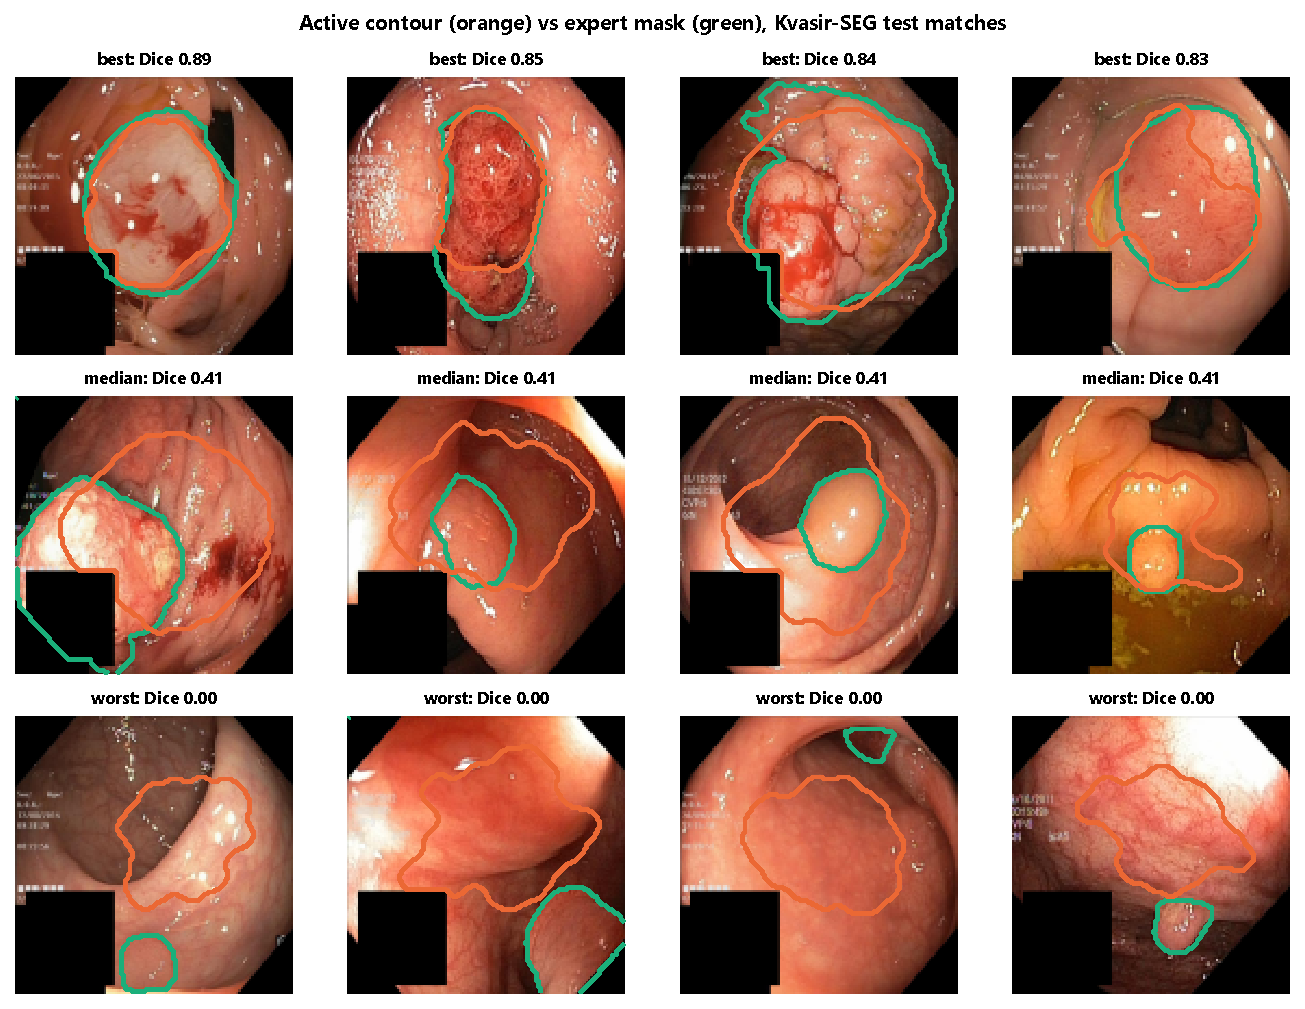
\includegraphics[width=\columnwidth]{ac_gallery.pdf}
\caption{Contour (orange) vs expert mask (green) on Kvasir-SEG test matches: best, median and worst by Dice. Failures are lumen/fold regions and small lesions.}
\label{fig:acgallery}
\end{figure}

\subsection{Classical baselines and feature controls}
Chance is a macro-F1 of \randF{}; the Lab-colour centroid heuristic reaches \heurF{} (polyp AUROC \heurAU{}).
LightGBM on global colour and texture features reaches \lgbGF{}; adding the contour features raises it to \lgbGACF{}.
\emph{However, the controls match or exceed the real contour:} replacing the contour by an image-independent central ellipse gives \lgbGEllF{},
and a contour borrowed from another image gives \lgbGShufF{}. What helps is therefore ``colour and texture inside versus outside a central region'', not the contour itself.
A linear probe on frozen DINOv2 embeddings reaches \dinoProbeF{}, above every hand-crafted pipeline.

\subsection{Deep backbones}
Table~\ref{tab:leaderboard} compares all models under one protocol. Fine-tuned ConvNeXt-T, EfficientNetV2-S, Swin-T and DINOv2 ViT-S/14 lie within about one to two points of each other
(macro-F1 \convnextF{}, \effnetF{}, \swinF{} and \dinoF{}), while the ResNet-50 recipe trails at \resnetF{}. Polyp-vs-rest AUROC is above 0.99 for all fine-tuned networks.
A soft-voting ensemble of the five backbones reaches \ensF{}.
\begin{table*}[t]
\centering
\caption{Held-out test performance (mean$\pm$SD over seeds; deep models $N{=}3$, classical $N{=}5$). Best per column in bold. ECE after temperature scaling.}
\label{tab:leaderboard}
\small
\begin{adjustbox}{max width=\linewidth}\begin{tabular}{lrrrrr}
\toprule
Model & Macro-F1 & Acc. & MCC & Polyp AUROC & ECE \\
\midrule
ResNet-50 & 0.8708{\scriptsize$\pm$0.0043} & 0.8712{\scriptsize$\pm$0.0045} & 0.8530{\scriptsize$\pm$0.0051} & 0.9916{\scriptsize$\pm$0.0017} & 0.0300{\scriptsize$\pm$0.0026} \\
EfficientNetV2-S & 0.9257{\scriptsize$\pm$0.0025} & 0.9258{\scriptsize$\pm$0.0025} & 0.9153{\scriptsize$\pm$0.0029} & \textbf{0.9957{\scriptsize$\pm$0.0004}} & 0.0256{\scriptsize$\pm$0.0035} \\
ConvNeXt-T & 0.9233{\scriptsize$\pm$0.0006} & 0.9235{\scriptsize$\pm$0.0006} & 0.9128{\scriptsize$\pm$0.0007} & 0.9931{\scriptsize$\pm$0.0029} & 0.0353{\scriptsize$\pm$0.0027} \\
Swin-T & 0.9327{\scriptsize$\pm$0.0045} & 0.9327{\scriptsize$\pm$0.0045} & 0.9232{\scriptsize$\pm$0.0051} & 0.9947{\scriptsize$\pm$0.0014} & 0.0306{\scriptsize$\pm$0.0050} \\
DINOv2 ViT-S/14 & \textbf{0.9344{\scriptsize$\pm$0.0058}} & \textbf{0.9343{\scriptsize$\pm$0.0058}} & \textbf{0.9250{\scriptsize$\pm$0.0066}} & 0.9916{\scriptsize$\pm$0.0015} & 0.0242{\scriptsize$\pm$0.0035} \\
ACG-ConvNeXt (full) & 0.9277{\scriptsize$\pm$0.0035} & 0.9279{\scriptsize$\pm$0.0035} & 0.9178{\scriptsize$\pm$0.0040} & 0.9900{\scriptsize$\pm$0.0013} & 0.0325{\scriptsize$\pm$0.0016} \\
ACG-ResNet-50 & 0.8560{\scriptsize$\pm$0.0103} & 0.8565{\scriptsize$\pm$0.0100} & 0.8363{\scriptsize$\pm$0.0114} & 0.9887{\scriptsize$\pm$0.0023} & 0.0353{\scriptsize$\pm$0.0049} \\
LightGBM $\cdot$ global colour/texture & 0.7507{\scriptsize$\pm$0.0037} & 0.7513{\scriptsize$\pm$0.0037} & 0.7160{\scriptsize$\pm$0.0042} & 0.9565{\scriptsize$\pm$0.0003} & 0.1285{\scriptsize$\pm$0.0011} \\
LightGBM $\cdot$ contour features only & 0.8063{\scriptsize$\pm$0.0029} & 0.8073{\scriptsize$\pm$0.0029} & 0.7804{\scriptsize$\pm$0.0033} & 0.9721{\scriptsize$\pm$0.0005} & 0.1450{\scriptsize$\pm$0.0036} \\
LightGBM $\cdot$ global + contour & 0.7954{\scriptsize$\pm$0.0045} & 0.7964{\scriptsize$\pm$0.0045} & 0.7678{\scriptsize$\pm$0.0052} & 0.9716{\scriptsize$\pm$0.0006} & 0.1310{\scriptsize$\pm$0.0056} \\
Logistic reg. $\cdot$ global + contour & 0.7763 & 0.7773 & 0.7458 & 0.9712{\scriptsize$\pm$0.0000} & 0.0308{\scriptsize$\pm$0.0000} \\
LightGBM $\cdot$ global + central-ellipse features (control) & 0.8003{\scriptsize$\pm$0.0028} & 0.8005{\scriptsize$\pm$0.0028} & 0.7721{\scriptsize$\pm$0.0032} & 0.9788{\scriptsize$\pm$0.0002} & 0.1303{\scriptsize$\pm$0.0027} \\
LightGBM $\cdot$ global + shuffled-contour features (control) & 0.7840{\scriptsize$\pm$0.0013} & 0.7847{\scriptsize$\pm$0.0014} & 0.7542{\scriptsize$\pm$0.0016} & 0.9695{\scriptsize$\pm$0.0004} & 0.1338{\scriptsize$\pm$0.0008} \\
RBF-SVM $\cdot$ global + contour & 0.7900 & 0.7905 & 0.7609 & 0.9749{\scriptsize$\pm$0.0000} & \textbf{0.0219} \\
Random forest $\cdot$ global + contour & 0.7658{\scriptsize$\pm$0.0044} & 0.7666{\scriptsize$\pm$0.0044} & 0.7338{\scriptsize$\pm$0.0051} & 0.9624{\scriptsize$\pm$0.0004} & 0.1079{\scriptsize$\pm$0.0044} \\
XGBoost $\cdot$ global + contour & 0.7947{\scriptsize$\pm$0.0045} & 0.7955{\scriptsize$\pm$0.0044} & 0.7667{\scriptsize$\pm$0.0051} & 0.9735{\scriptsize$\pm$0.0011} & 0.1179{\scriptsize$\pm$0.0054} \\
Linear probe $\cdot$ frozen DINOv2 & 0.8889{\scriptsize$\pm$0.0000} & 0.8890 & 0.8732 & 0.9951{\scriptsize$\pm$0.0000} & 0.0354 \\
Random guess & 0.1311 & 0.1311 & 0.0070 & 0.4947 & 0.2116 \\
Class prior (majority) & 0.0279 & 0.1255 & 0.0000 & 0.4917 & 0.0000 \\
Heuristic $\cdot$ nearest Lab-colour centroid & 0.4762 & 0.4793 & 0.4066 & 0.8372 & 0.2669 \\
\bottomrule
\end{tabular}\end{adjustbox}
\end{table*}

\subsection{Does contour guidance help? (RQ1, RQ2)}
Table~\ref{tab:ablation} and Fig.~\ref{fig:forest} give the ablation on ConvNeXt-T. Plain ConvNeXt-T scores \plainF{}$\pm$\plainFSD{}. The full ACG model scores \acgF{}$\pm$\acgFSD{}
($\Delta=$ \acgDelta{}, 95\,\% CI \acgDeltaLo{} to \acgDeltaHi{}, Holm-adjusted $p=$ \acgPHolm{}).
\textbf{The difference is not statistically supported}, and neither are the shuffled-image control (\shufDelta{}) and the ellipse control (\ellDelta{}): all three overlap.
Non-contour global features alone give \gfeatDelta{}, the largest and only nominally significant bootstrap difference, which does not survive Holm correction (adjusted $p=$ \gfeatPHolm{}).
Seed-level paired $t$-tests with $N{=}3$ are fragile (the plain model's seed SD is only \plainFSD{}, which inflates standardised effect sizes) and are therefore reported in the repository but not relied on.
Generality: ACG on ResNet-50 scores \resacgF{}\,$\pm$\,\resacgFSD{} against \resnetF{} for plain ResNet-50.
\begin{table*}[t]
\centering
\caption{Ablation on ConvNeXt-T ($N{=}3$ seeds). $\Delta$: seed-averaged macro-F1 difference to the plain baseline with 95\,\% paired-bootstrap interval over test images; $p$: Holm-adjusted bootstrap p-value.}
\label{tab:ablation}
\small
\begin{adjustbox}{max width=\linewidth}\begin{tabular}{lrrrl r}
\toprule
Variant & Macro-F1 & Acc. & Polyp AUROC & $\Delta$ [95\,\% CI] & $p_\mathrm{Holm}$ \\
\midrule
ConvNeXt-T (plain) & 0.9233{\scriptsize$\pm$0.0006} & 0.9235 & 0.9931 & +0.0000 -- & -- \\
+ global hand-crafted features & 0.9295{\scriptsize$\pm$0.0035} & 0.9295 & 0.9927 & +0.0062 [+0.0013, +0.0111] & 0.072 \\
+ contour pooling & 0.9264{\scriptsize$\pm$0.0037} & 0.9264 & 0.9934 & +0.0031 [-0.0015, +0.0075] & 0.380 \\
+ contour features & 0.9288{\scriptsize$\pm$0.0003} & 0.9289 & 0.9932 & +0.0055 [+0.0004, +0.0106] & 0.180 \\
ACG-ConvNeXt (full) & 0.9277{\scriptsize$\pm$0.0035} & 0.9279 & 0.9900 & +0.0045 [-0.0004, +0.0091] & 0.296 \\
full, shuffled contours (control) & 0.9275{\scriptsize$\pm$0.0015} & 0.9276 & 0.9912 & +0.0043 [-0.0010, +0.0093] & 0.354 \\
full, central ellipse (control) & 0.9267{\scriptsize$\pm$0.0067} & 0.9268 & 0.9908 & +0.0035 [-0.0017, +0.0085] & 0.380 \\
\bottomrule
\end{tabular}\end{adjustbox}
\end{table*}
\begin{figure}[t]
\centering
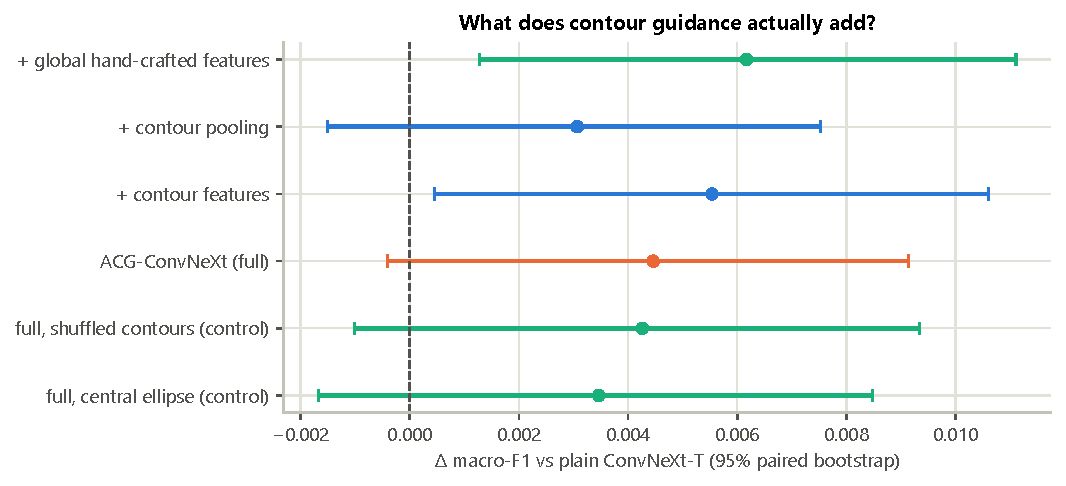
\includegraphics[width=\columnwidth]{ablation_forest.pdf}
\caption{Difference in macro-F1 to plain ConvNeXt-T with 95\,\% paired-bootstrap intervals (unadjusted). The full model and both image-independent controls are indistinguishable.}
\label{fig:forest}
\end{figure}

\subsection{Shortcuts and leakage (RQ3)}
Despite the strong metadata shortcuts (Section~\ref{sec:data}), a ConvNeXt-T trained on \emph{naive} full frames (no crop, no artefact mask) reaches \naiveF{}\,$\pm$\,\naiveFSD{},
statistically equal to the canonical \plainF{}: the shortcuts separate upper-GI from colon, which pixels already do, while the remaining errors are within-region pairs where neither shortcut carries information.
Training and testing on a \emph{random} split with the same sizes gives \randsplitF{}\,$\pm$\,\randsplitFSD{} (different test images, so not paired), consistent with the modest \randLeakPct{} near-duplicate overlap measured in the audit.

\subsection{Calibration and conformal prediction (RQ5)}
Temperature scaling reduces ECE from \eceRaw{} to \eceCal{}. Validation-calibrated conformal sets reach only \confCovVal{} coverage at a nominal 95\,\%,
because the validation split was reused for early stopping, temperature and threshold and is therefore optimistic. Calibrating on a random half of the test \emph{scene groups} and evaluating on the other half
(200 repeats) restores coverage: \confCov{}\,$\pm$\,\confCovSD{}, mean set size \confSize{}, \confSingle{} singleton sets (Fig.~\ref{fig:cal}).
For polyp-vs-rest, at a miss cost five times a false alarm, the 0.5 threshold has expected cost \costHalf{} per image against \costYouden{} for the validation-Youden threshold and \costOpt{} for the validation cost-optimal threshold:
thresholds tuned on the optimistic validation split did not beat the default.
\begin{figure}[t]
\centering
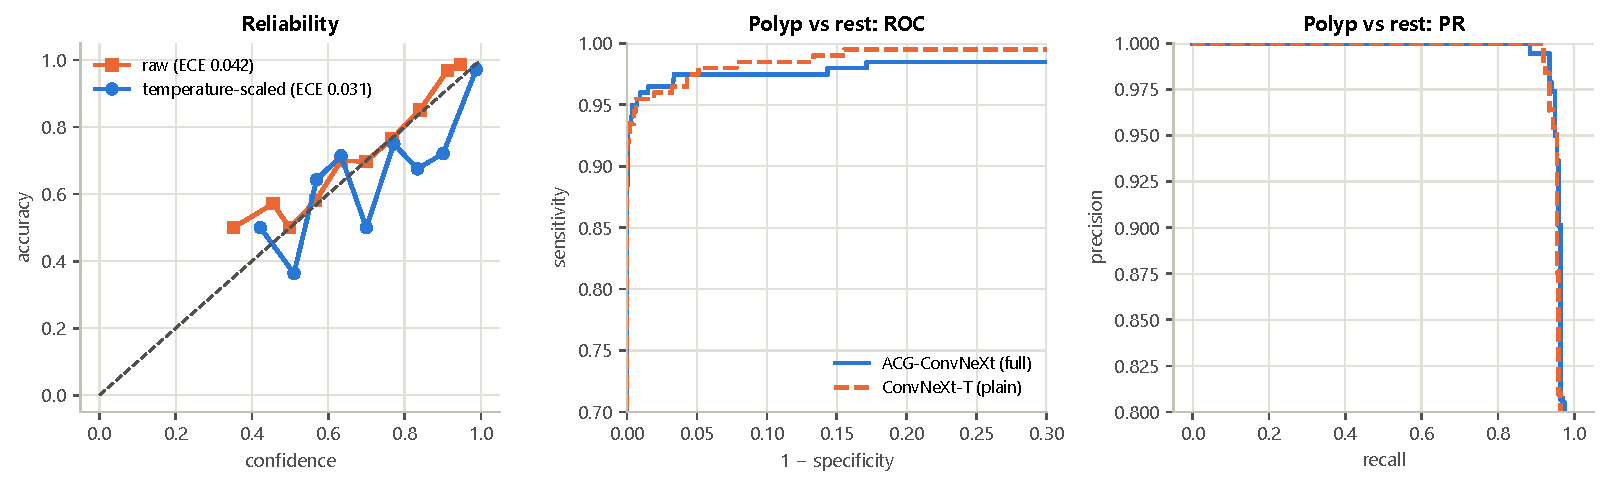
\includegraphics[width=\columnwidth]{calibration_roc_pr.pdf}
\caption{Reliability before/after temperature scaling, and polyp-vs-rest ROC and PR curves (seed 0).}
\label{fig:cal}
\end{figure}

\subsection{Error analysis}
Of \nErrors{} test errors (\errRate{}), \errPairs{} fall into two confusable pairs (esophagitis$\leftrightarrow$z-line and dyed-lifted$\leftrightarrow$dyed-resection-margins; Fig.~\ref{fig:conf}).
\errFlagged{} of the errors involve images flagged by confident learning, against \corrFlagged{} of correct predictions, so a large share of the residual error is label ambiguity rather than model failure.
We inspected the 36 most confident errors (a visual judgement by a non-clinician, not an adjudication): 17 are esophagitis$\leftrightarrow$z-line, 7 are dyed-lifted$\leftrightarrow$resection-margin, 7 are ``polyp'' frames with no distinct visible lesion (the clinically important group, only 2 of which are flagged), and 5 are other colitis/cecum mixes; 26 of the 36 are flagged.
The most confident errors (Fig.~\ref{fig:err}) show craters with dye that are plausible for either dyed class, homogeneous mucosa labelled ``polyp'' with no visible lesion, and z-line frames with inflammation.
Accuracy is \accColonScope{} on colon-scope (720$\times$576) frames and \accUpperScope{} on larger-format upper-GI frames; the worst class accuracy is \worstClassAcc{}.
\begin{figure}[t]
\centering
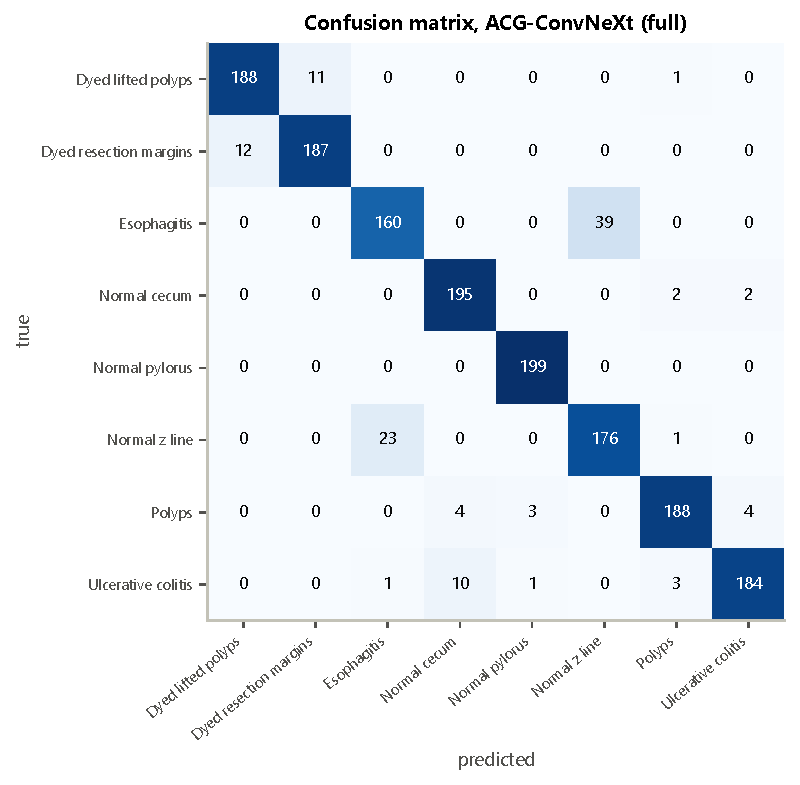
\includegraphics[width=0.85\columnwidth]{confusion_matrix.pdf}
\caption{Confusion matrix of the seed-ensembled ACG-ConvNeXt on the test split.}
\label{fig:conf}
\end{figure}
\begin{figure*}[t]
\centering
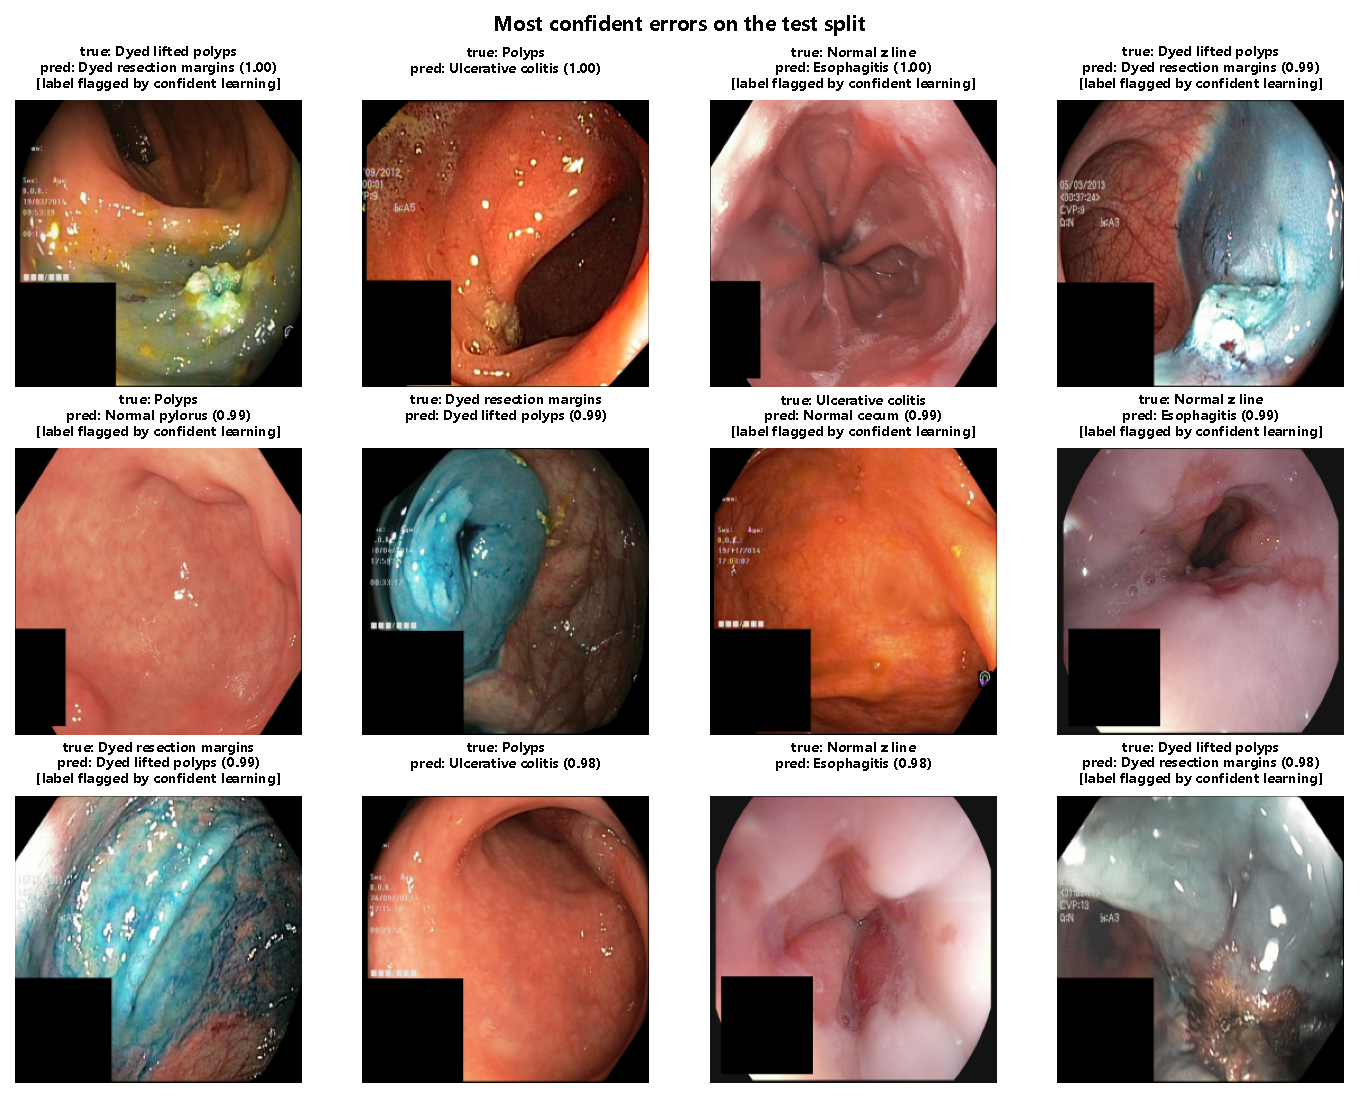
\includegraphics[width=0.8\textwidth]{error_gallery.pdf}
\caption{The twelve most confident errors, with confident-learning flags.}
\label{fig:err}
\end{figure*}

\subsection{Data efficiency, robustness and interpretability (RQ4)}
\paragraph{Data efficiency (RQ4).}
Training on 10\,\%, 25\,\%, 50\,\% and 100\,\% of the training split gives macro-F1 \lcNoneTen{}, \lcNoneTwentyFive{}, \lcNoneFifty{}, \lcNoneFull{} for the plain model and
\lcAcgTen{}, \lcAcgTwentyFive{}, \lcAcgFifty{}, \lcAcgFull{} for ACG-ConvNeXt (Fig.~\ref{fig:lc}). The curves overlap: guidance does not help more when data are scarce.
\begin{figure}[t]
\centering
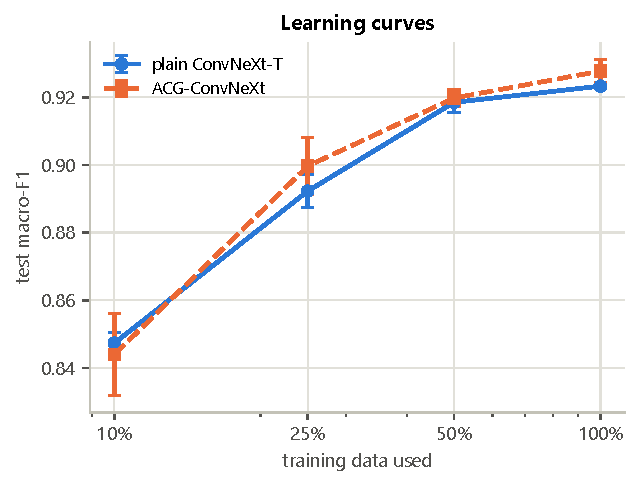
\includegraphics[width=0.8\columnwidth]{learning_curves.pdf}
\caption{Learning curves (mean $\pm$ SD over 3 seeds).}
\label{fig:lc}
\end{figure}

\paragraph{Learning-rate sensitivity.}
Deep hyper-parameters were not tuned per variant. For seed 0, the plain model scores \lrNoneHalf{}, \lrNoneDef{} and \lrNoneDouble{} at half, default and double learning rate, and the guided model \lrAcgHalf{}, \lrAcgDef{} and \lrAcgDouble{}:
changing the learning rate moves macro-F1 by as much as any ablation effect, and the default rate was evidently not optimal for the plain model.
The guided model's seed-0 score at the doubled rate looked like a clear gain, but that rate was singled out after seeing test results, so we replicated it as an exploratory, post hoc check with three seeds per variant:
plain \lrTwoPlain{}\,$\pm$\,\lrTwoPlainSD{}, guided \lrTwoAcg{}\,$\pm$\,\lrTwoAcgSD{} ($\Delta=$ \lrTwoDelta{}, 95\,\% CI \lrTwoLo{} to \lrTwoHi{}, unadjusted bootstrap $p=$ \lrTwoP{}).
Both variants improve over the default rate and the gap between them is not distinguishable from zero, so the null conclusion holds at the better learning rate as well. A fully fair comparison would tune every variant on validation data, which we did not do.

\paragraph{Robustness.}
On \robN{} stratified test frames, JPEG compression at quality 50 lowers accuracy from \robPlainClean{} to \robPlainJpegFifty{} for the plain model, but only from \robAcgClean{} to \robAcgJpegFifty{} for the guided model (Fig.~\ref{fig:rob}).
At quality 10 the figures are \robPlainJpegTen{} against \robAcgJpegTen{}, and under Gaussian blur with $\sigma=3$\,px \robPlainBlurThree{} against \robAcgBlurThree{}.
\emph{The controls reproduce this advantage:} shuffled-image contours give \robShufJpegFifty{} and the central ellipse \robEllJpegFifty{} at quality 50, and global features alone give \robGfeatJpegFifty{}.
Robustness therefore comes from supplying colour and texture statistics computed on the pixels, not from the contour's alignment with the lesion.
\begin{figure*}[t]
\centering
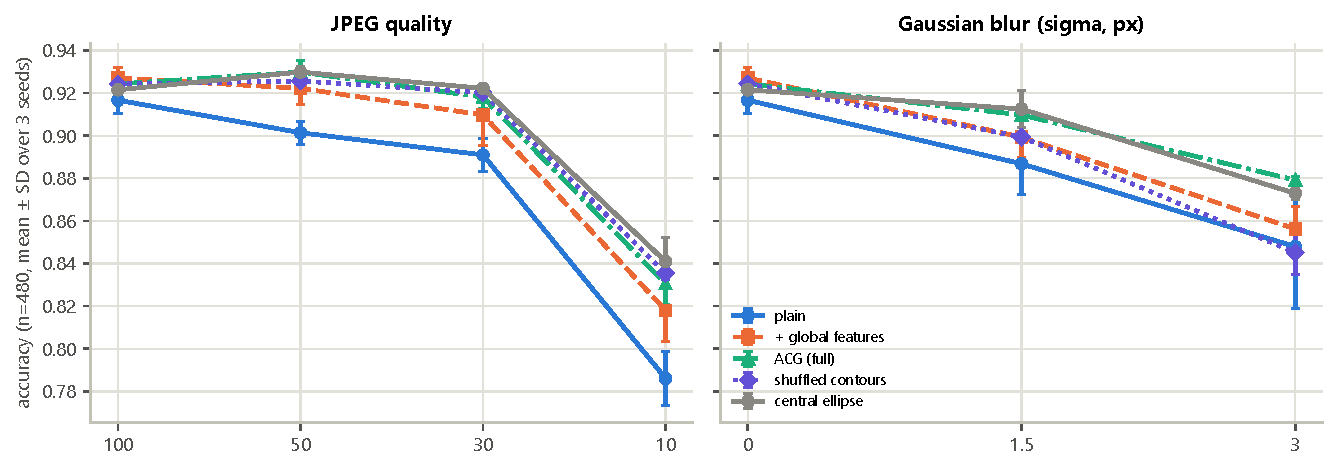
\includegraphics[width=0.7\textwidth]{robustness_multiseed.pdf}
\caption{Accuracy under JPEG compression and Gaussian blur (mean $\pm$ SD over 3 seeds, 480 test frames; contours and features recomputed on the degraded pixels).}
\label{fig:rob}
\end{figure*}

\paragraph{Interpretability.}
\emph{Grad-CAM against expert masks.} Using the polyp-class Grad-CAM on the 176 Kvasir-SEG test-split polyps, the CAM maximum lies inside the expert mask for \plainPoint{} of frames for the plain model and \acgPoint{} for the guided model;
the top-20\,\% CAM pixels overlap the mask with IoU \plainCamIoU{} and \acgCamIoU{}. The CAM maximum falls inside the active contour for \plainCamInAC{} and \acgCamInAC{} of frames.
With $n=176$ these differences are within sampling noise: the guided network does not attend to lesions more accurately than the plain one.
\emph{TreeSHAP} on LightGBM with global and contour features attributes \shapRegion{} of the total importance to inside/outside colour and texture (region) features and \shapGlobal{} to global features, but only \shapShape{} to contour shape and \shapBoundary{} to boundary features:
the geometry of the contour carries little information.
\emph{Layer-wise linear probes} on ConvNeXt-T stages give macro-F1 \lwPreOne{} (pretrained) and \lwFtOne{} (fine-tuned) at stage~1, \lwPreThree{} and \lwFtThree{} at stage~3, and \lwPreFour{} and \lwFtFour{} at stage~4:
fine-tuning mostly reshapes the last two stages.



\section{Discussion}
\paragraph{Why did the contour not help?}
Three observations point the same way. (i) The contour is a weak localiser (Dice \acDice{}, over-segmenting \acOverSeg{}$\times$), so the spatial prior it provides is only slightly better than a central ellipse.
(ii) A fine-tuned ConvNeXt, Swin or DINOv2 backbone already localises the evidence it needs; the Grad-CAM peaks of the plain and guided models fall inside the expert polyp mask equally often (Section~V-H).
(iii) The residual error is dominated by label ambiguity rather than by missing localisation: \errPairs{} of errors lie in two confusable pairs and \errFlagged{} involve flagged labels, so there is little headroom for any prior.
The small positive differences we see ($\le0.6$ points) track \emph{extra hand-crafted inputs}, whether or not they involve a contour, and the shuffled and ellipse controls reproduce them.
In the classical setting the same pattern holds: contour features beat global features (\lgbGF{} to \lgbGACF{}), but a central ellipse does better still (\lgbGEllF{}).

\paragraph{What the study does establish.}
(1) Kvasir v2 contains duplicates, a label contradiction, strong acquisition shortcuts and substantial label ambiguity, all quantified here.
(2) Under one audited protocol, modern fine-tuned backbones reach macro-F1 of 0.92--0.93 (ensemble \ensF{}); published Kvasir accuracies are not directly comparable because class subsets, splits and preprocessing differ and we could not verify those protocols, so we make no claim about ranking against them. Our own control shows a random split changes macro-F1 by about one point (\randsplitF{} against \plainF{}, different test images) and the polyp AUROC far more.
(3) Calibration is easy to get wrong in practice: validation data reused for model selection under-covered conformal sets (\confCovVal{} against 95\,\%), and a group-aware split of the test set repaired it.
(4) A random split can mislead through the AUROC (\randsplitAU{} against \plainAU{}) more than through accuracy.

\paragraph{Threats to validity and limitations.}
\emph{Single centre, no patient IDs:} scene groups reduce but cannot exclude patient-level leakage, and nothing here tests transfer to other scopes or hospitals.
\emph{Three seeds:} bootstrap intervals over test images capture sampling uncertainty given those seeds; seed-level tests are fragile and are not used for inference.
\emph{One recipe for all variants:} deep hyper-parameters were not tuned per variant, which is fair across variants but may under-serve any of them (a learning-rate sweep is reported in the repository).
\emph{Unsupervised contour only:} a learned, interactive or video-propagated prior could behave differently; we make no claim about those.
\emph{Overlay text} inside the field of view was not removed.
\emph{Not clinical:} no prospective validation, no regulatory claim, and the dataset terms exclude commercial use without written permission.

\paragraph{Future work.}
Learned lesion priors trained on Kvasir-SEG, patient-level splits on datasets that provide identifiers, external validation, and video-based consistency are the natural next steps.

\section{Conclusion}
An unsupervised active-contour prior, evaluated with controls, did not measurably improve fine-tuned deep classification of Kvasir findings, while the audit, the leakage-aware protocol, the calibrated and conformal outputs and the error analysis are reusable.
We report the null result as a result, with the code, splits and statistics needed to challenge it.


\section*{Reproducibility and Ethics}
All code, configurations, split hashes and logs are in the accompanying repository; \texttt{scripts/run\_experiments.ps1}
rebuilds every table and figure. Kvasir and Kvasir-SEG are used under their research-and-education terms; the datasets are not redistributed, and the few frames shown in figures are attributed illustrations.
This is a research prototype, not a medical device, and must not be used for clinical decisions.

\bibliographystyle{IEEEtran}
\bibliography{references}
\end{document}
